\chapter{The v2 synthetic generator}
\label{chap:v2gen}

The v2 generator (single file
\texttt{data-gen/generate\_custom\_dataset.py}) implements every
recommendation produced by \cref{chap:reanalysis}. The CSV output
schema (\texttt{time\_step, gamma\_dose, is\_anomaly}) is unchanged, so
the training pipeline of \cref{chap:archi} does not need to be
touched.

\section{What changed, item by item}
\label{sec:v2-changes}

\paragraph{Background noise: AR(1) replaces IID Gaussian.} The
high-frequency residual is now generated as
\begin{equation}
    r_t = \varphi\, r_{t-1} + \varepsilon_t,
    \quad \varepsilon_t \overset{\text{iid}}{\sim}
        \mathcal{N}(0, \sigma_\varepsilon^2),
    \qquad \varphi = 0.86,
    \quad \sigma_\varepsilon = 1.12,
    \label{eq:v2-ar1}
\end{equation}
exactly the values fitted in \cref{eq:ar1-noise,tab:reanal-noise}. The
state $r_t$ is propagated across the $50\,000$-sample writing chunks,
so the AR(1) memory is not broken at chunk boundaries. The marginal
standard deviation is still $\sigma_r \approx 2.30$, matching the v1
generator and the real data, but the local texture of a $512$-sample
window is now substantially smoother on the few-sample scale.
\Cref{fig:noise-texture} shows the texture difference explicitly.

\begin{figure}[H]
    \centering
    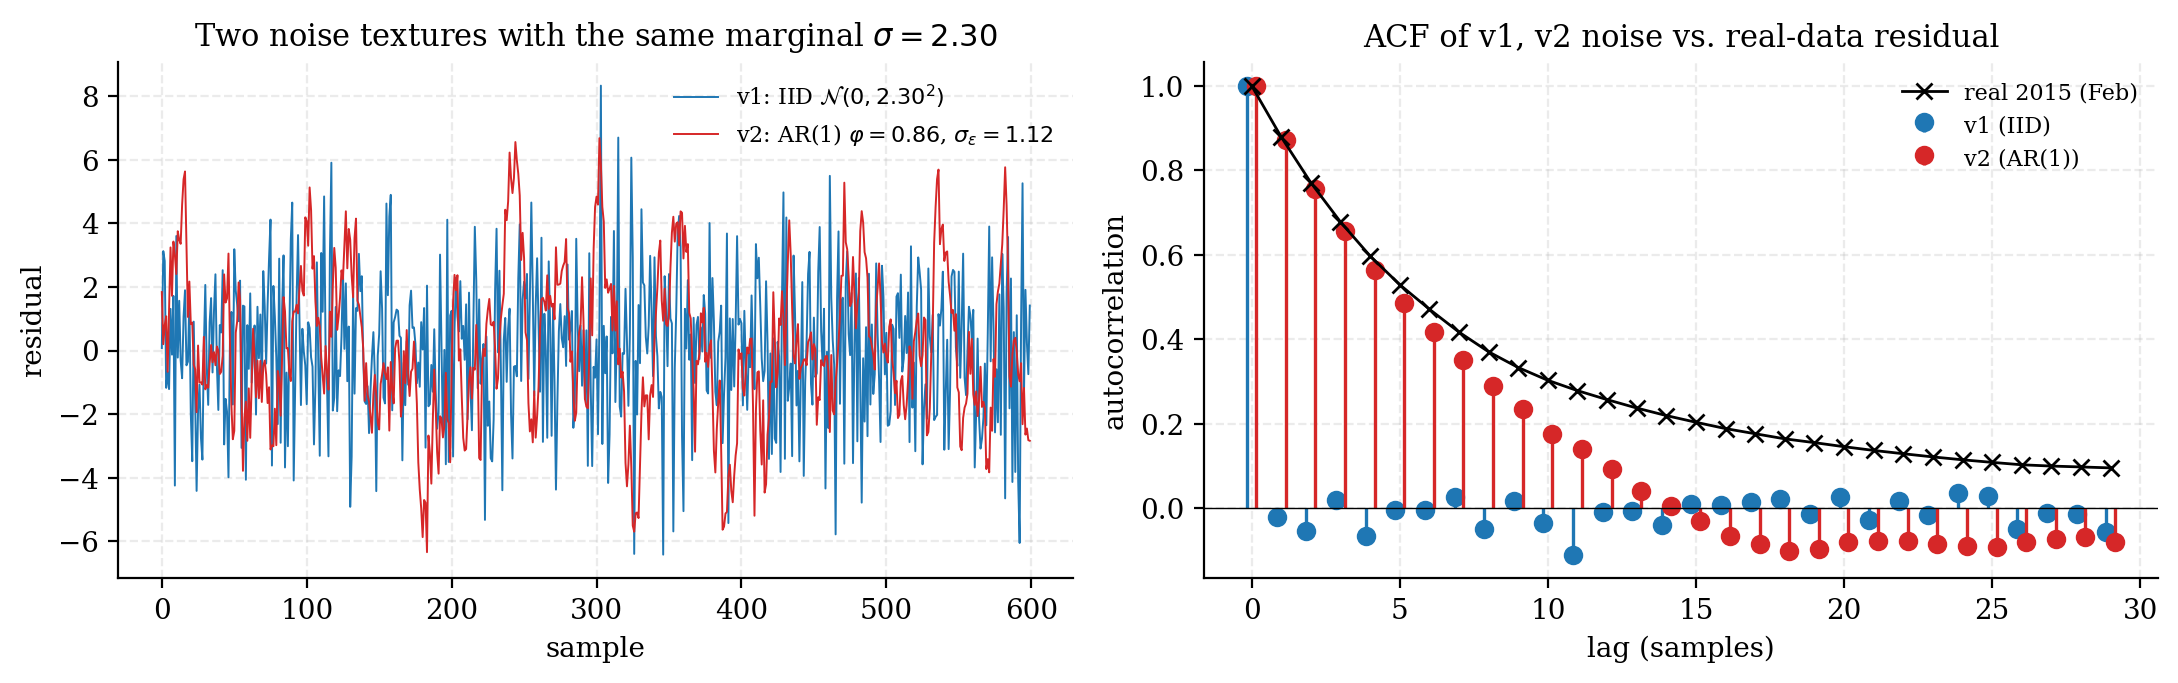
\includegraphics[width=\linewidth]{figures/noise_texture_comparison}
    \caption{\textbf{Left}: $600$ samples of IID Gaussian noise
    ($\sigma = 2.30$, v1) and of AR(1) noise ($\varphi = 0.86$,
    $\sigma_\varepsilon = 1.12$, v2) sharing the same marginal
    standard deviation. The AR(1) trace is visibly smoother on the
    few-sample scale. \textbf{Right}: the corresponding empirical
    ACFs, alongside the real-data residual ACF (black). The v2 noise
    matches the real ACF; the v1 noise does not.}
    \label{fig:noise-texture}
\end{figure}

\paragraph{Baseline: tuned OU + per-recording offset.} The OU process
is retained but its parameters are re-tuned to $\theta = 2.5 \cdot
10^{-5}$ and $\sigma_{\mathrm{OU}} = 0.007$, giving a stationary
baseline standard deviation of $\sim 1$ count and a typical
$40$k-sample drift range of $\sim 4$ counts (the empirical wide-scale
range of \cref{tab:reanal-drift}). The global mean is sampled per
recording around $\mu = 99.3$ with $\pm 1.5$ jitter, matching the
empirical month-to-month variation in \cref{tab:real-stats}.

\paragraph{Anomaly count and density.} The injection grid samples
$M \in [1\,300, 1\,700]$ anomalies per $10^{7}$-sample dataset, a
density of $\sim 1.5$ events per $10\text{k}$ samples. Slightly above
the empirical $1.05$ from \cref{sec:reanalysis-labels} to give the
network a few extra training examples, but well below the v1 density
of $\sim 7$ events per $10\text{k}$ samples. This is the single
largest fix relative to v1, and the one that addresses the
prior-shift cause of \cref{sec:v1-fail-causes}.

\paragraph{Anomaly amplitudes: log-uniform $[15, 40]$ counts
(absolute).} The hand-labelled events have peak amplitudes (above the
local MA-4320 baseline) in the range $[11.2, 36.8]$ counts. The v2
generator samples amplitudes log-uniformly in $[15, 40]$ counts: the
lower bound is raised above the empirical minimum because amplitudes
below $\sim 15$ counts are not separable from the AR(1)+OU background
texture at the $\sigma \approx 2.3$ noise level, and were degrading
the training signal-to-noise ratio without representing a detectable
population. The upper bound is set slightly above the empirical
maximum.

\paragraph{Anomaly durations: log-uniform $[30, 1000]$ samples.} The
empirical range is $[32, 1014]$ samples and the bulk of the
distribution sits below $400$. The v2 $[30, 1000]$ range covers the
full empirical span. The v1 range of $[200, 800]$ missed both the very
short events of June (durations of $32$--$55$ samples) and the long
events of October (up to $1\,014$ samples).

\paragraph{Polarity: $100\%$ positive.} All $17$ hand-labelled events
are positive excursions. The v1 generator was already
polarity-symmetric in spirit (positive amplitudes only) so no change
was required, but this is now explicitly justified by the labels
rather than inherited from the templates.

\paragraph{Template family: three, not six.} The \texttt{M},
\texttt{bell\_sq} and \texttt{square} templates were dropped: no
labelled real event has the multi-peak structure of \texttt{M}, the
plateau-with-bumps profile of \texttt{bell\_sq}, or the sustained
square profile of \texttt{square}. The retained family
(\texttt{bell}, \texttt{fast\_ascend}, \texttt{fast\_descend}) covers
the observed shapes, in roughly $53\%$, $29\%$, $18\%$ proportion
(\cref{sec:reanalysis-labels}). The generator samples the three
templates uniformly (\emph{i.e.}\ $33\%$ each); the discrepancy is
small enough that no explicit biasing is applied.

\begin{figure}[H]
    \centering
    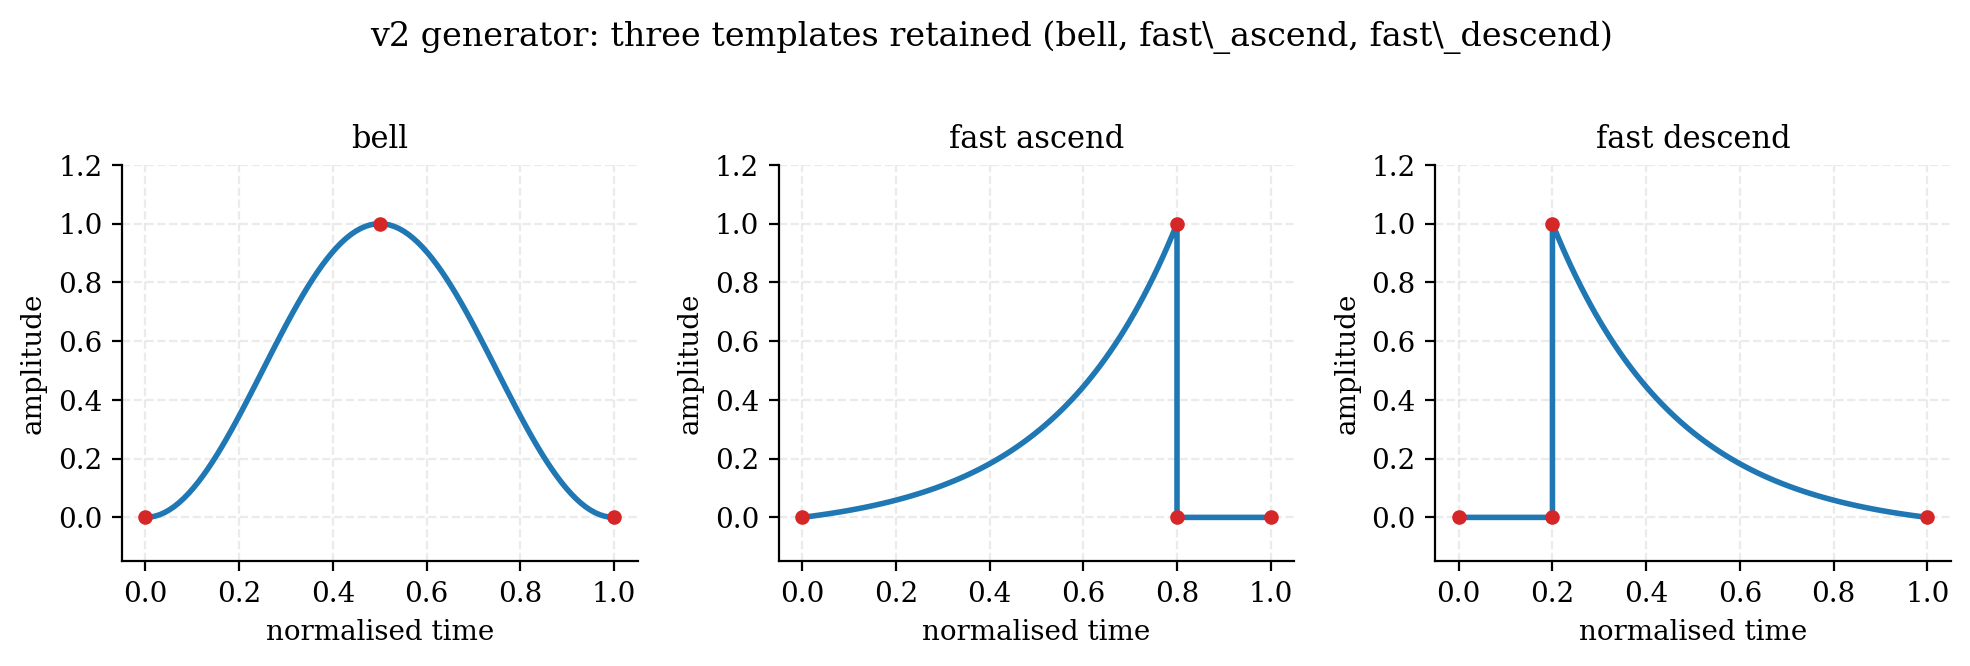
\includegraphics[width=\linewidth]{figures/v2_anomaly_templates}
    \caption{The three v2 templates --- the only shapes that have an
    empirical counterpart in the hand-labelled events of
    \cref{sec:reanalysis-labels}.}
    \label{fig:v2-templates}
\end{figure}

\begin{figure}[H]
    \centering
    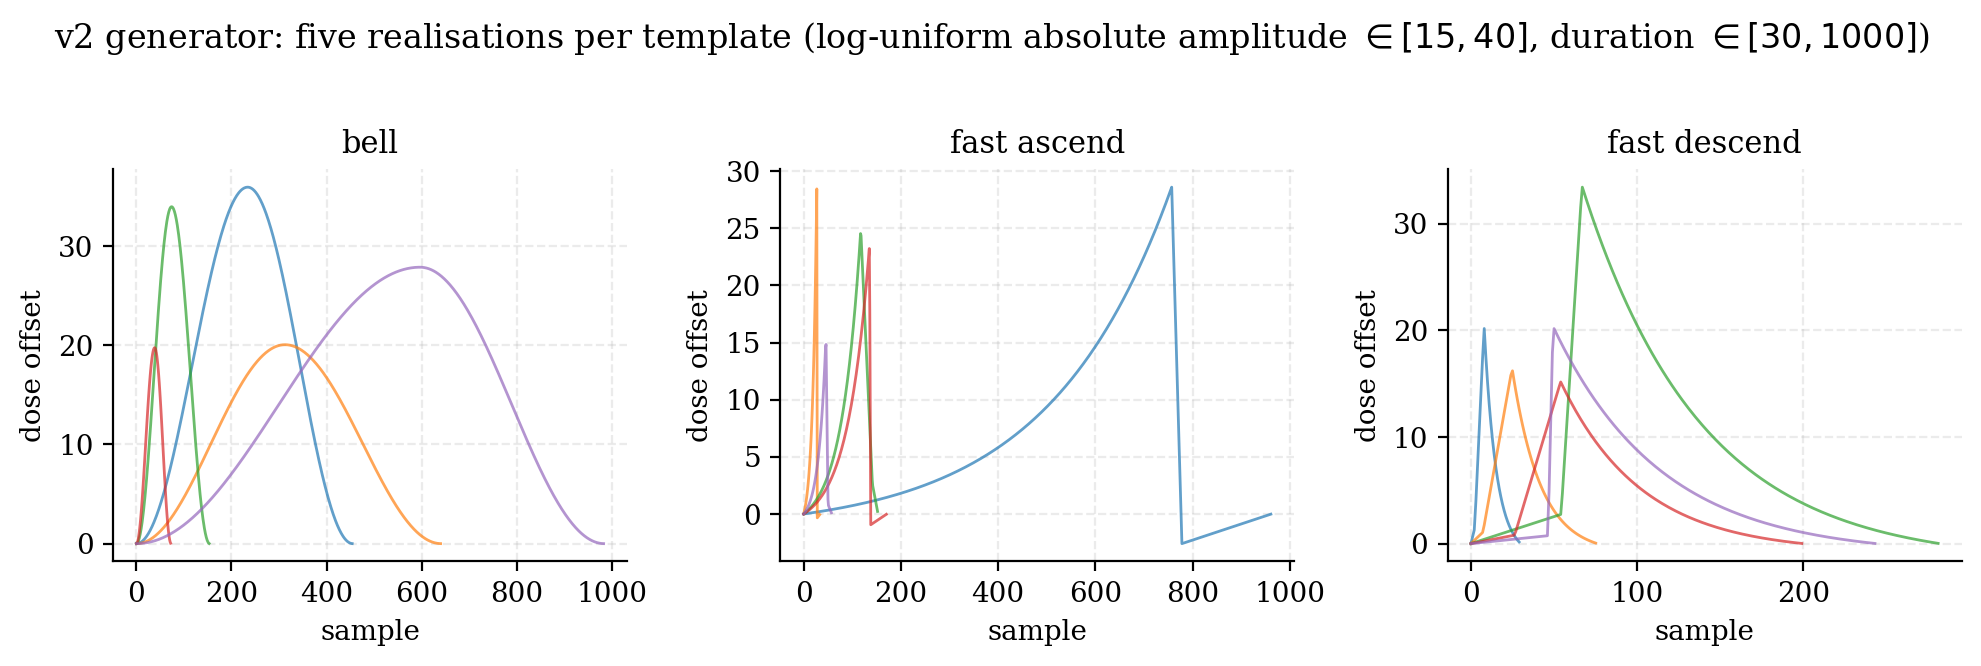
\includegraphics[width=\linewidth]{figures/v2_template_deformation}
    \caption{Five stochastic realisations of each v2 template, drawn
    with log-uniform amplitudes in $[15, 40]$ counts and log-uniform
    durations in $[30, 1000]$ samples.}
    \label{fig:v2-deformation}
\end{figure}

\section{The v2 generator algorithm}
\label{sec:v2-algo}

The end-to-end algorithm is structurally identical to the v1 one
(\cref{sec:v1-gen-algo}); only the background generation step and the
parameter ranges differ. In pseudocode:
\begin{enumerate}[leftmargin=*, itemsep=0.2em]
    \item Sample a per-recording global mean
    $\mu \sim \mathcal{U}(99.3 \pm 1.5)$.
    \item Decide the total number of anomalies
    $M \in [1\,300, 1\,700]$ and their injection grid (uniform spacing
    with $\pm 400$ random jitter).
    \item Pre-generate all anomaly waveforms: for each injection point,
    sample a template uniformly from the three v2 templates, sample
    $(\text{amp}, \text{period}) \sim \text{Log-Uniform}(15, 40) \times
    \text{Log-Uniform}(30, 1000)$ and a deformation variance
    $\nu \sim \mathcal{U}(0.02, 0.10)$; deform and interpolate the
    template into a dense curve.
    \item Generate the background in $50\,000$-sample chunks. For each
    chunk, simulate an OU step ($\theta = 2.5 \cdot 10^{-5}$,
    $\sigma_{\mathrm{OU}} = 0.007$) and an AR(1) step
    ($\varphi = 0.86$, $\sigma_\varepsilon = 1.12$), \emph{both} with
    state continuation across chunk boundaries to preserve the AR(1)
    memory and the OU drift.
    \item Add each anomaly curve on top of the background at its
    injection index and label every output point with the anomaly's
    class (or $0$ if the per-point contribution falls below the
    threshold).
\end{enumerate}

\section{The v2 dataset used in this report}
\label{sec:v2-final-dataset}

The v2 results in \cref{chap:results,chap:robustness,chap:v2real} are
all computed on a single $N = 10^{7}$-sample dataset; with the v2
density target, this contains roughly $1\,500$ anomalies. The first
$100$k samples of the dataset are shown in \cref{fig:v2-synth-preview}.

\begin{figure}[H]
    \centering
    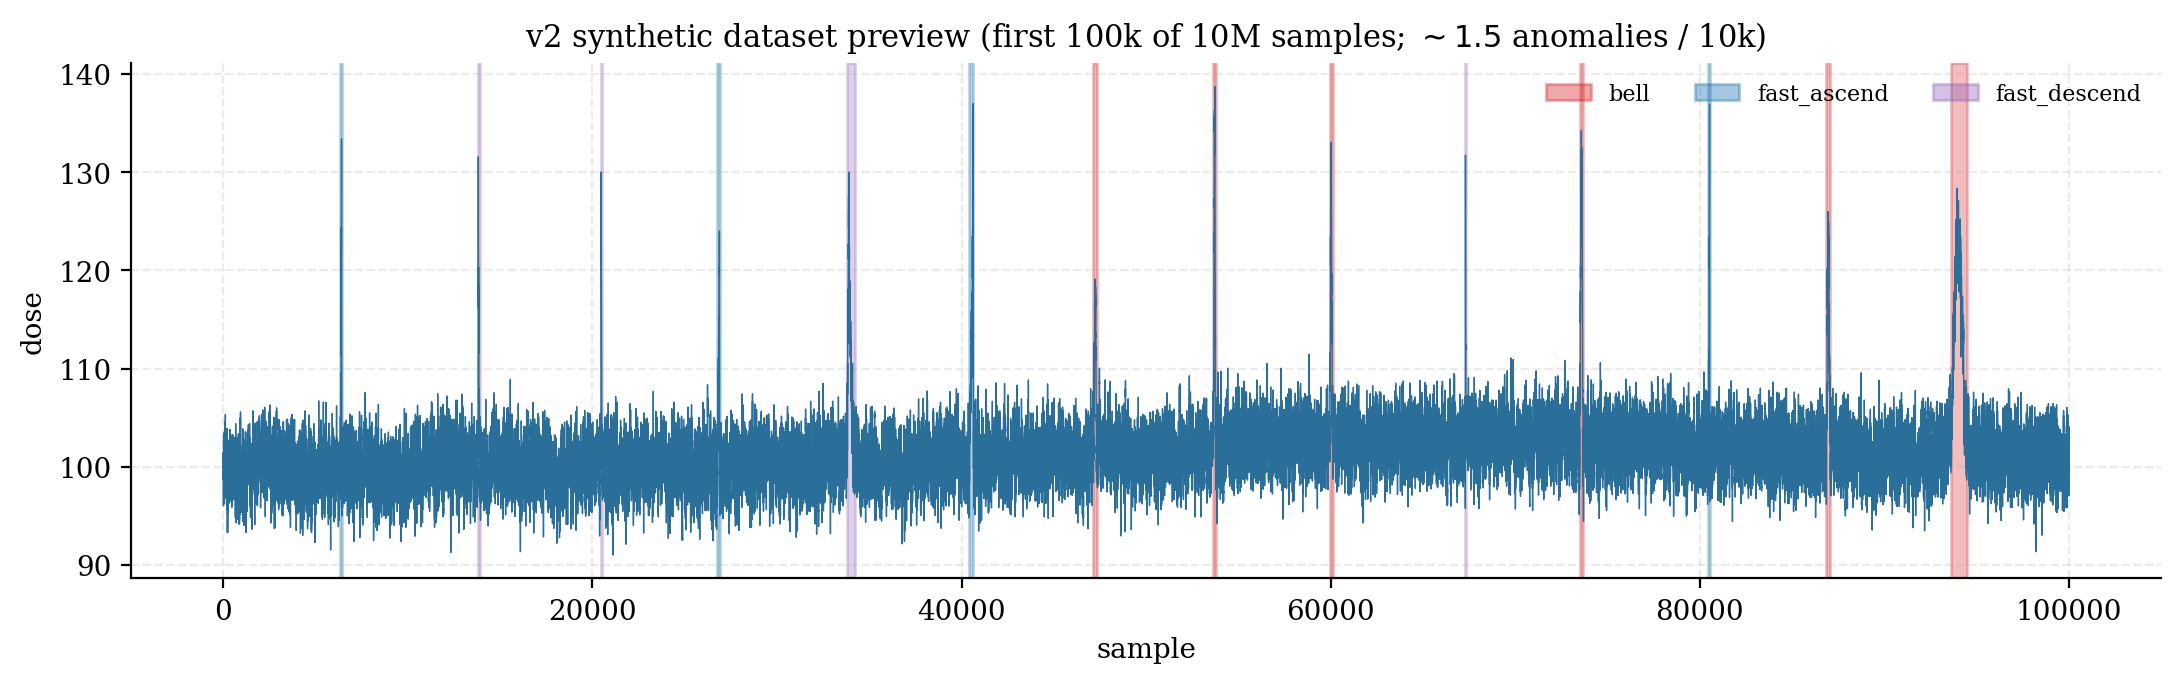
\includegraphics[width=\linewidth]{figures/v2_synthetic_preview}
    \caption{First $100\,000$ samples (of $10^{7}$) of the v2 synthetic
    dataset. Anomaly spans are coloured by class. Note the sparse
    injection compared to \cref{fig:v1-synth-preview}: $\sim 15$ events
    in this view, against four in the v1 $30$k-sample preview.}
    \label{fig:v2-synth-preview}
\end{figure}

\Cref{fig:v1-vs-v2-synth} puts the two iterations side by side on
$30\,000$-sample slices.

\begin{figure}[H]
    \centering
    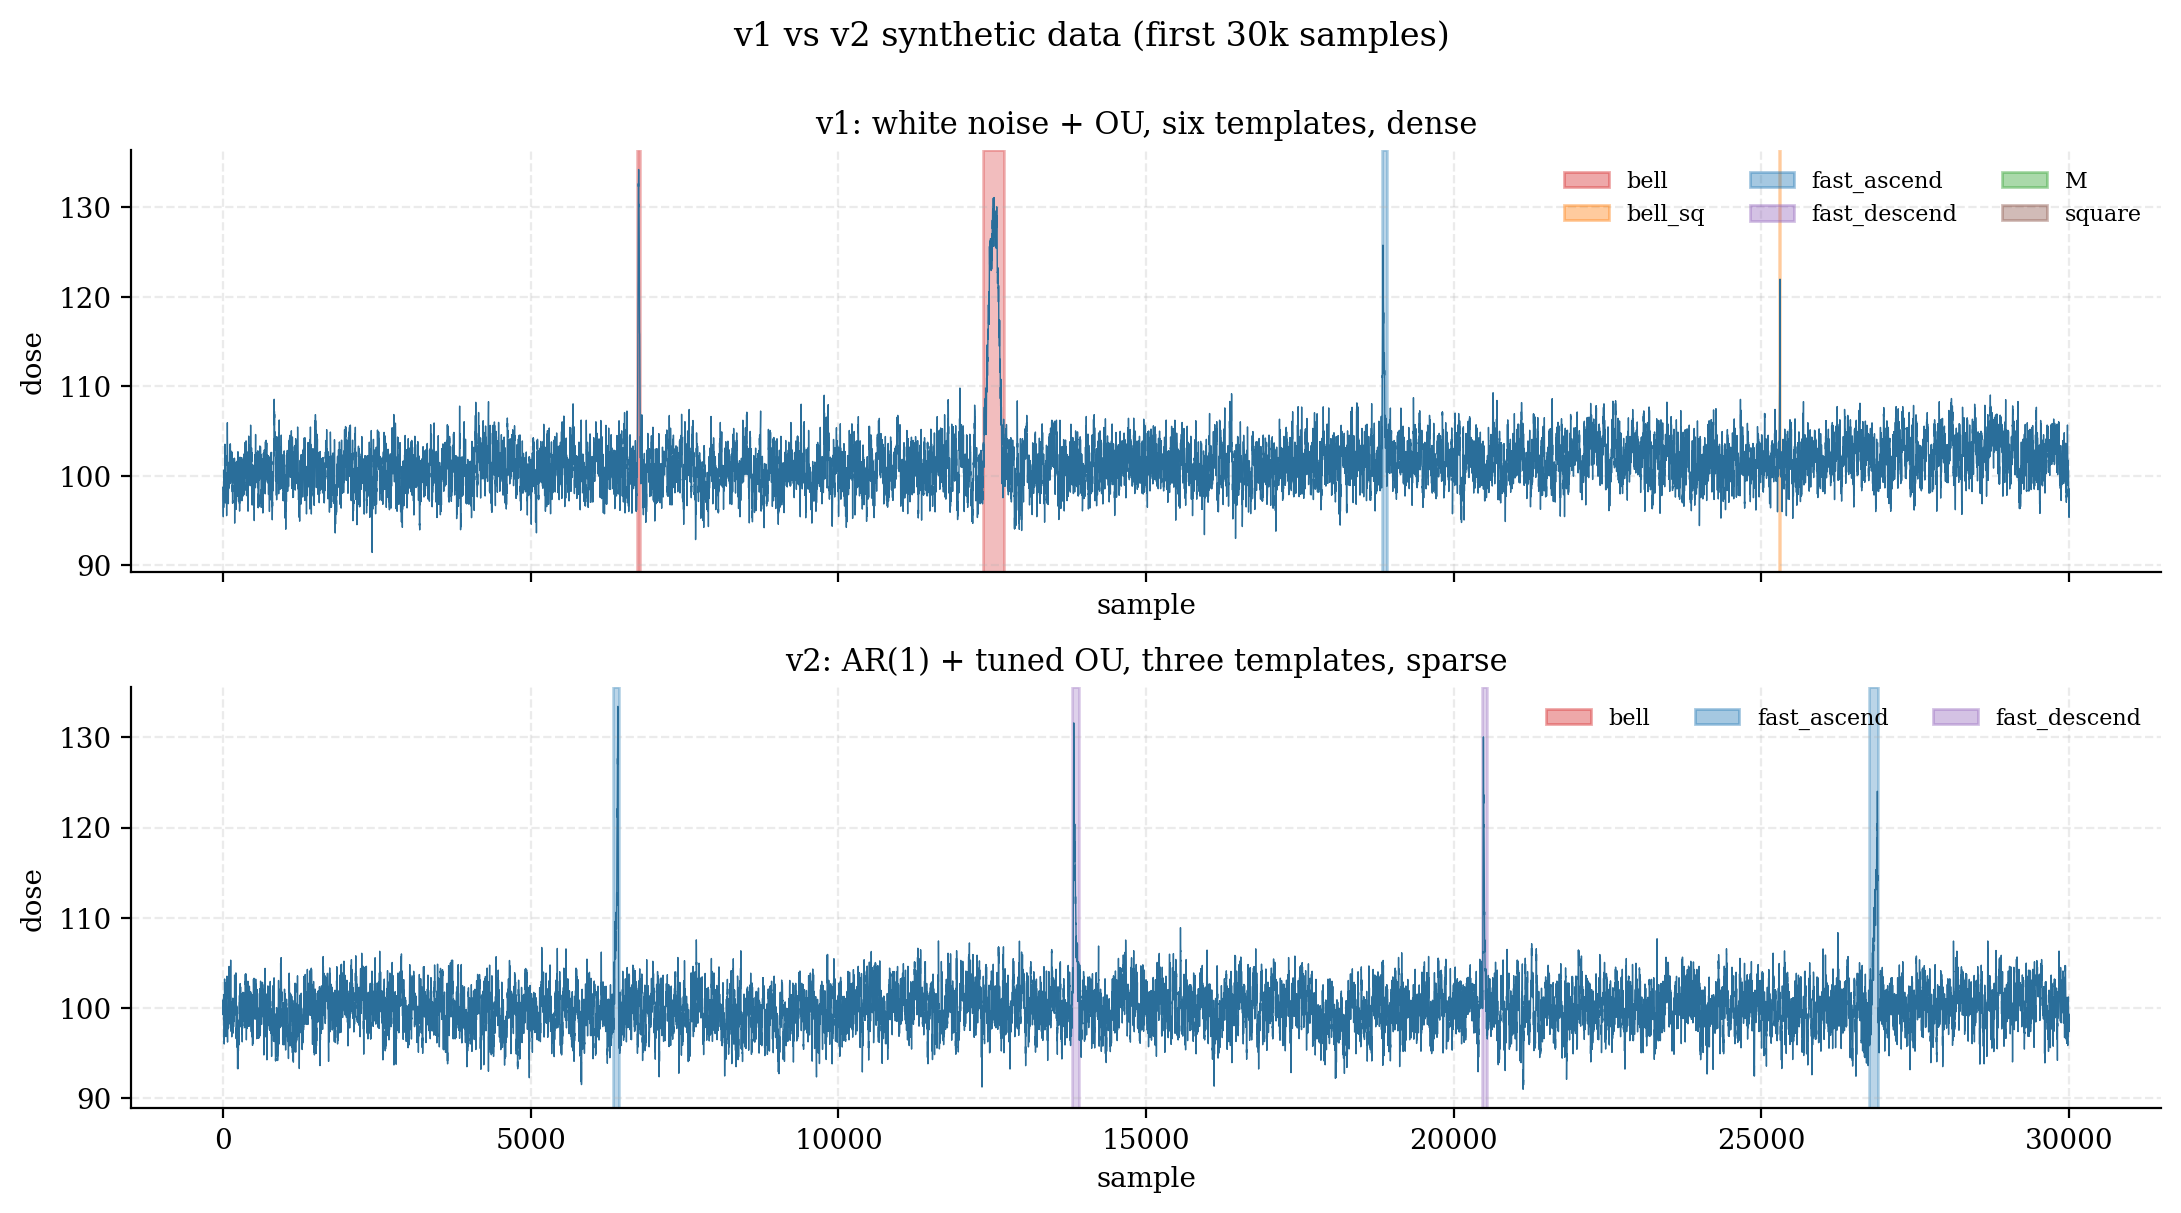
\includegraphics[width=\linewidth]{figures/v1_vs_v2_synthetic}
    \caption{v1 vs v2 synthetic data on the same window size. v1 has
    four visible bumps; v2 has zero. The marginal noise standard
    deviation is the same ($\sigma \approx 2.3$), but the local
    texture of v2 is smoother because of the AR(1) memory.}
    \label{fig:v1-vs-v2-synth}
\end{figure}

\section{Acceptance test}
\label{sec:v2-accept}

Running \texttt{analyze\_noise\_model.py} on a $50\,000$-sample chunk
of the v2 output reproduces:
\begin{itemize}[leftmargin=*, itemsep=0.2em]
    \item the AR(1) coefficient $\varphi \approx 0.86$ (by
    construction);
    \item the innovation standard deviation
    $\sigma_\varepsilon \approx 1.12$ (by construction);
    \item the marginal residual standard deviation
    $\sigma_r \approx 2.30$ (algebraic consequence);
    \item Ljung--Box on AR(1) innovations: the synthetic AR(1) output
    \emph{passes} the whiteness test, in contrast to the real signal
    where AR(1) is formally rejected due to a residual
    $\varphi_2 \approx -0.02$ that the generator does not attempt to
    reproduce. This is the expected behaviour for an exactly AR(1)
    process and is not a defect of the generator;
    \item linear-trend slope distribution centred on zero, with
    standard deviation matching the empirical $\sim 10^{-4}$ counts
    per sample, produced by the OU mechanism rather than an explicit
    linear term.
\end{itemize}

\paragraph{Why the linear-trend term is folded into the OU.} The v2
generator does not implement an explicit per-recording linear slope.
A linear term added to a $10^{7}$-sample synthetic signal would
diverge by orders of magnitude over the dataset length, far beyond
what the OU process can produce. The re-tuned $(\theta,
\sigma_{\mathrm{OU}})$ pair was chosen so that the OU drift over
$40$k samples (the length of a single real recording) has the right
amplitude distribution; over $10^{7}$ samples the OU process stays
bounded around $\mu$, which is what we want for training.

In practice the convolutional stem cannot tell ``OU drift with the
right variance'' apart from ``OU drift with the same variance plus a
small linear term''; both look like a slowly varying baseline at the
window scale.

\section{What v2 still does not fix}
\label{sec:v2-remaining}

The $17$ hand labels are sufficient to constrain the marginal
distributions (amplitude, duration, polarity, shape family) and to
validate the inference qualitatively, but they are not sufficient to
compute event-level precision and recall on real data: there is no
labelled real test set against which to score an inference run. The
v2 generator is also still ``binary'' in spirit: a window either
contains a clean templated event or pure stationary background, with
no class for ``unknown but not Normal''. The two limitations
compound, and they both argue that the next round of work should be
expert labelling of the real recordings (yielding both a real test
set and a more refined set of empirical event distributions), not
further generator tuning.

This is the last planned iteration of the data-generation pipeline.
The next chapter trains the three architectures on v2 and reports the
event-level results on the synthetic test segment.
